\documentclass{article}
%-----Packages-----
%\usepackage{fullpage}
\usepackage{booktabs}
\usepackage{amsmath}
\usepackage{amssymb}
\usepackage{amsthm}
\usepackage{etoolbox}
\usepackage{hyperref}
\usepackage{float}
\usepackage{graphicx}
%\usepackage{subcaption}
\usepackage{epsfig} 

\usepackage{subfigure}

\usepackage{comment} 
\usepackage[margin =  1.25in]{geometry}

\graphicspath{{./figures/}}
%\graphicspath{{C:/Users/Will/Desktop/}}

\usepackage{hyperref}
\hypersetup{colorlinks = true,linktoc = all,linkcolor = blue}


\usepackage{enumitem}
\usepackage{latexsym}
\usepackage{mathrsfs} 
\usepackage{enumitem}
\usepackage{latexsym}
\usepackage{mathrsfs} 
\usepackage[all,arc]{xy} 
\usepackage{amsmath,mathtools}
\usepackage{multicol}
\usepackage{siunitx,lipsum}
\usepackage{esint} 
\usepackage{parallel}
\usepackage{titlesec}
\usepackage{thmtools}
\usepackage[T1]{fontenc}
\usepackage[]{algorithm2e}
\usepackage{float}

%-----Bold Math Capitals-----
\newcommand{\bA}{\mathbf{A}}
\newcommand{\bB}{\mathbf{B}}
\newcommand{\bC}{\mathbf{C}}
\newcommand{\bD}{\mathbf{D}}
\newcommand{\bE}{\mathbf{E}}
\newcommand{\bF}{\mathbf{F}}
\newcommand{\bG}{\mathbf{G}}
\newcommand{\bH}{\mathbf{H}}
\newcommand{\bI}{\mathbf{I}}
\newcommand{\bJ}{\mathbf{J}}
\newcommand{\bK}{\mathbf{K}}
\newcommand{\bL}{\mathbf{L}}
\newcommand{\bM}{\mathbf{M}}
\newcommand{\bN}{\mathbf{N}}
\newcommand{\bO}{\mathbf{O}}
\newcommand{\bP}{\mathbf{P}}
\newcommand{\bQ}{\mathbf{Q}}
\newcommand{\bR}{\mathbf{R}}
\newcommand{\bS}{\mathbf{S}}
\newcommand{\bT}{\mathbf{T}}
\newcommand{\bU}{\mathbf{U}}
\newcommand{\bV}{\mathbf{V}}
\newcommand{\bW}{\mathbf{W}}
\newcommand{\bX}{\mathbf{X}}
\newcommand{\bY}{\mathbf{Y}}
\newcommand{\bZ}{\mathbf{Z}}

%-----Blackboard Bold Math Capitals-----
\newcommand{\bbA}{\mathbb{A}}
\newcommand{\bbB}{\mathbb{B}}
\newcommand{\bbC}{\mathbb{C}}
\newcommand{\bbD}{\mathbb{D}}
\newcommand{\bbE}{\mathbb{E}}
\newcommand{\bbF}{\mathbb{F}}
\newcommand{\bbG}{\mathbb{G}}
\newcommand{\bbH}{\mathbb{H}}
\newcommand{\bbI}{\mathbb{I}}
\newcommand{\bbJ}{\mathbb{J}}
\newcommand{\bbK}{\mathbb{K}}
\newcommand{\bbL}{\mathbb{L}}
\newcommand{\bbM}{\mathbb{M}}
\newcommand{\bbN}{\mathbb{N}}
\newcommand{\bbO}{\mathbb{O}}
\newcommand{\bbP}{\mathbb{P}}
\newcommand{\bbQ}{\mathbb{Q}}
\newcommand{\bbR}{\mathbb{R}}
\newcommand{\bbS}{\mathbb{S}}
\newcommand{\bbT}{\mathbb{T}}
\newcommand{\bbU}{\mathbb{U}}
\newcommand{\bbV}{\mathbb{V}}
\newcommand{\bbW}{\mathbb{W}}
\newcommand{\bbX}{\mathbb{X}}
\newcommand{\bbY}{\mathbb{Y}}
\newcommand{\bbZ}{\mathbb{Z}}
\newcommand{\g}[1]{g(#1)}
%-----Script Math Capitals-----
\newcommand{\sA}{\mathscr{A}}
\newcommand{\sB}{\mathscr{B}}
\newcommand{\sC}{\mathscr{C}}
\newcommand{\sD}{\mathscr{D}}
\newcommand{\sE}{\mathscr{E}}
\newcommand{\sF}{\mathscr{F}}
\newcommand{\sG}{\mathscr{G}}
\newcommand{\sH}{\mathscr{H}}
\newcommand{\sI}{\mathscr{I}}
\newcommand{\sJ}{\mathscr{J}}
\newcommand{\sK}{\mathscr{K}}
\newcommand{\sL}{\mathscr{L}}
\newcommand{\sM}{\mathscr{M}}
\newcommand{\sN}{\mathscr{N}}
\newcommand{\sO}{\mathscr{O}}
\newcommand{\sP}{\mathscr{P}}
\newcommand{\sQ}{\mathscr{Q}}
\newcommand{\sR}{\mathscr{R}}
\newcommand{\sS}{\mathscr{S}}
\newcommand{\sT}{\mathscr{T}}
\newcommand{\sU}{\mathscr{U}}
\newcommand{\sV}{\mathscr{V}}
\newcommand{\sW}{\mathscr{W}}
\newcommand{\sX}{\mathscr{X}}
\newcommand{\sY}{\mathscr{Y}}
\newcommand{\sZ}{\mathscr{Z}}
\newcommand{\defeq}{\mathrel{\mathop:}=}
\newcommand\DistTo{\xrightarrow{
		\,\smash{\raisebox{-0.65ex}{\ensuremath{\scriptstyle\sim}}}\,}}
\newcommand{\secref}[1]{\S\ref{#1}}
%-----Redefined Commands-----
\newcommand{\p}[1]{\left(#1\right)}
\newcommand{\uv}[1]{\mathbf{\hat{#1}}}
\newcommand{\ml}[1]{\mathbb{#1}}
\newcommand{\ov}[1]{\overline{#1}}
\newcommand{\ab}[1]{\left|#1\right|}
\renewcommand{\sb}[1]{\left[#1\right]}
\renewcommand{\vec}[1]{\mathbf{#1}}
\newcommand{\ginv}[1]{#1^{-1}}
\newcommand{\cinv}[1]{\frac{\overline{#1}}{\norm{#1}^2}}
\newcommand{\finv}[1]{\frac{1}{#1}}
\newcommand{\zmodnz}[1]{\bbZ/#1\bbZ}
%\renewcommand{\phi}{\varphi}
\providecommand{\abs}[1]{\lvert #1 \rvert}
\providecommand{\norm}[1]{\lVert #1 \rVert}
\providecommand{\x}{\times}
\providecommand{\ra}{\rightarrow}
\providecommand{\arr}{\longrightarrow}
\providecommand{\lpn}[2]{\norm{#1}_{l^#2}} 
\providecommand{\lpns}[3]{\norm{#1}_{l^{#2}(#3)}}
\providecommand{\Lpn}[2]{\norm{#1}_{L^{#2}}}
\providecommand{\Lpns}[3]{\norm{#1}_{L^{#2}(#3)}}
\providecommand{\sbn}[2]{\norm{#1}_{W^{(1,#2)}}}


\renewcommand{\v}[1]{\mathbf{#1}}
\renewcommand{\vec}[1]{\mathbf{#1}}
\newcommand{\pwrzero}{\sum\limits_{n=0}^{\infty} a_nz^n} 
\newcommand{\pwrat}[1]{\sum\limits_{n=0}^{\infty} a_n(z-#1)^n} 
\newcommand{\ser}[3]{\sum\limits_{#1 = #2}^{#3}}
\newcommand{\seri}[1]{\sum\limits_{#1}}

%Operators%
\newcommand{\normsq}[1]{\norm{#1}^2}
\newcommand{\partialpartial}[2]{\frac{\partial #1}{\partial #2}}  
\newcommand{\pp}[2]{\frac{\partial#1}{\partial#2}}
\providecommand{\lintegral}[2]{\int\limits_{#1}^{#2}} 
\providecommand{\fintegral}[1]{\int\limits_{#1}}
\providecommand{\sintegral}[1]{\fint\limits_{#1}}
\providecommand{\lac}[1]{\Delta#1}
\providecommand{\lacc}[2]{\Delta(#1)(#2)}
\providecommand{\vlac}[1]{(\nabla^2)} 
\providecommand{\grad}[1]{\nabla#1} 
\providecommand{\expt}[1]{\langle #1 \rangle}
\providecommand{\diff}[1]{\partial_{#1}}
\providecommand{\fdiff}[2]{(\partial_{#1}#2)}
\providecommand{\dtime}{\frac{d}{dt}}
\providecommand{\tdiff}[1]{\frac{d}{d#1}}
\providecommand{\fnl}[1]{\hat{\v{#1}}}
\providecommand{\pb}[2]{\{#1,#2\}}
\providecommand{\ip}[2]{\langle #1, #2 \rangle}
\providecommand{\trace}[1]{\text{Tr}(#1)}
\providecommand{\lip}[1]{\text{Lip}(#1)}
\providecommand{\hsn}[1]{\norm{#1}_{H^1}}
\providecommand{\hsno}[1]{\norm{#1}_{H^{1}_0}}
\providecommand{\htn}[1]{\norm{#1}_{H^2_0(U)}}


%Constant Symbols, Typesetting% 
\providecommand{\hbar}{\hslash}
\providecommand{\bk}{k_B}
\providecommand{\qmt}{\frac{\hbar^2}{2m}}
\renewcommand{\v}[1]{\mathbf{#1}}
\renewcommand{\vec}[1]{\mathbf{#1}}
\newcommand{\mc}[1]{\mathcal{#1}}
\providecommand{\radi}{R_{n,l}(r)}
\providecommand{\radfi}{u_{n,l}(r)}
\providecommand{\sphi}{Y_{l,m}(\theta,\varphi)}
\providecommand{\Psii}{\Psi_{n,l,m}}
\providecommand{\fdind}[3]{#1_{#2,#3}}
\providecommand{\ftind}[4]{#1_{#2,#3,#4}} 
\providecommand{\bs}[1]{\boldsymbol{#1}}
\providecommand{\support}[1]{\text{supp}(#1)} 
\providecommand{\mum}{\mu^{-}}
\providecommand{\mup}{\mu^{+}}
\providecommand{\lup}{\lambda^{+}}
\providecommand{\lum}{\lambda^{-}}
\providecommand{\nup}{\nu^{+}}
\providecommand{\nums} {\nu^{-}}
\providecommand{\linfty}[1]{\norm{#1}_{\infty}}
\providecommand{\posf}{f^{+}}
\providecommand{\negf}{f^{-}}
\providecommand{\essup}{\text{ess sup}}
\providecommand{\dual}[1]{#1^{\star}}
\providecommand{\dnorm}[1]{\norm{#1}_{\dual{E}}}
\providecommand{\wsto}{\stackrel{\star}{\rightharpoonup}}
\providecommand{\wto}{\rightharpoonup}
\providecommand{\Image}{\text{Im}}
\providecommand{\testfunctions}{C^{\infty}_C}
\providecommand{\holder}[1]{[#1]_{C^{\alpha}}} 
\providecommand{\aff}{\text{aff}}
\providecommand{\conv}{\text{conv}\ }
\providecommand{\MSE}{\text{MSE}}

%Objects%
\renewcommand{\phi}{\varphi}
\providecommand{\abs}[1]{\lvert #1 \rvert}
\providecommand{\norm}[1]{\lVert #1 \rVert}
\providecommand{\x}{\times}
\providecommand{\ra}{\rightarrow}
\providecommand{\arr}{\longrightarrow}
\providecommand{\lpm}[1]{\sL^{#1}(X,\sM,\mu)}
\providecommand{\ddz}{\frac{d}{dz}}
\newcommand{\cvec}[2]{\begin{pmatrix} #1 \\ #2 \end{pmatrix}}
\newcommand{\dmat}[4]{\begin{pmatrix} #1 & #2 \\ #3 & #4  \end{pmatrix}}
\newcommand{\spinx}{\frac{\hbar}{2}\begin{pmatrix} 0 & 1 \\ 1 & 0  \end{pmatrix}}
\newcommand{\spiny}{\frac{\hbar}{2}\begin{pmatrix} 0 & -i \\ i & 0  \end{pmatrix}}
\newcommand{\spinz}{\frac{\hbar}{2}\begin{pmatrix} 1 & 0 \\  0 & -1 \end{pmatrix}}
\newcommand{\obra}[1]{\langle #1 \vert }
\newcommand{\oket}[1]{\vert#1\rangle}
\newcommand{\inpd}[2]{\langle #1 \vert #2\rangle}
\newcommand{\ketbra}[2]{\oket{#1}\obra{#2}}
\newcommand{\ket}[1]{\vert #1 \rangle}
\newcommand{\bra}[1]{\langle #1 \vert} 
\providecommand{\seq}[2]{\{#1_{#2}\}_{#2 \in \bbZ_+}}
\providecommand{\acol}[1]{\{#1_\alpha\}}
\providecommand{\col}[3]{\{#1_{#2}\}_{#2 \in #3}}
\providecommand{\limsups}[3]{\bigcap_{#1 = 1}^{\infty} \bigcup_{#2 \geq #1} #3_{#2}} 
\providecommand{\dictorder}{<_d}
\providecommand{\aunion}[1]{\bigcup_{#1}}  
\providecommand{\aint}[1]{\bigcap_{#1}}
\providecommand{\ball}[2]{B(#1,#2)} 
\providecommand{\mball}[3]{B_{#3}(#1,#2)}
\providecommand{\Lp}[1]{\sL^{#1}(d\mu)}
\providecommand{\lpr}[2]{\sL^{#1}(\bbR^{#2},dm)}
\providecommand{\cont}[1]{\sC(#1)}
\providecommand{\contcs}[1]{\sC_C (#1)}
\providecommand{\weakstar}{\text{weak}^{\star}}
\providecommand{\cinfty}{C^{\infty}}
\newcommand{\eval}[2]{\vert^{#1}_{#2}}
\renewcommand{\div}{\text{div}}
\newcommand{\osc}{\text{osc}}
\newtheorem*{Proposition}{Proposition}
\newtheorem*{Remark}{Remark}
\newtheorem*{definition}{Definition}
\newtheorem*{lemma}{Lemma}
\newtheorem*{Theorem}{Theorem}
\newtheorem*{cor}{Corollary}
\newtheorem*{note}{Note}
\newtheorem*{claim}{Claim}
\newtheorem*{fact}{Fact}
\newtheorem*{Ex}{Example}
\newtheorem{Question}{Question}
\theoremstyle{remark} 


\numberwithin{equation}{subsection}
\AfterEndEnvironment{claim}{\noindent\ignorespaces}

\setcounter{tocdepth}{2}


%\title{ORNL-CAM: Running Project Notes}
%\author{William Porteous}
%\date{22 October 2019}

\begin{document} 
	
	%\maketitle
	
\begin{center}
	\textbf{Miscellaneous Results}
	\\[0.05in]
	Updated: \today 
\end{center}

\tableofcontents


\section{Framework: Choices Made}

\begin{enumerate} 
	\item \textbf{Sampling the Realizable Domain:} $\epsilon$-rejection along boundary curves plus uniform-in-alpha grid. N = 1,2.\\ 

	\item \textbf{Unified Training Routine:} Inputs and outputs for these models have been unified. Multiple loss combinations vailable, including 
	[h,$\boldsymbol{\alpha}$,$\vec{u}$].\\
	
	\item \textbf{Comparison Framework}: Comparison within the context of the M$_N$ solution routine includes a notion of efficiency. We may adjust hyperparameters, data-set, and network size in order to compare the accuracy and efficiency of resulting networks.\\
\end{enumerate}

\section{To Do}:
\begin{enumerate}
\item \textbf{Grid Search:} Grid search and comparison for different choices of networks and training penalties. \\ 

\item \textbf{Comparison with Modest N}: How do the models perform in high dimensional closure (with uniform sampling in alpha, where possible). 

\item \textbf{Sampling Strategy}: These models are defined in higher dimension but we cannot train and test them without data. This requires a more intelligent sampling than uniform-plus-rejection. 
\begin{itemize}
	\item Steffen's Undergrad - Monte Carlo
	\item Uniform Distance to Boundary Curves 
\end{itemize}
[h,$\alpha$,$\vec{u}$].\\
\end{enumerate} 
	


\section{Network Error Performance: Training and Testing Results}

\subsection{Training Loss Curves}

\begin{figure}[H]
	\subfigure[ECNN-15by2]{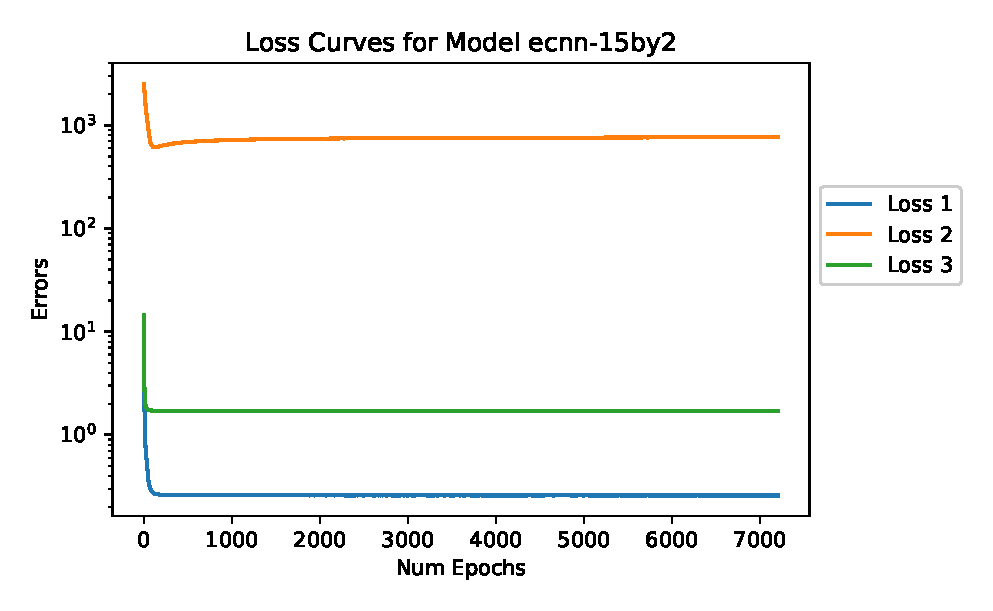
\includegraphics[width = 0.48\textwidth]{ecnn15by2}}
	\subfigure[ICNN-15by2]{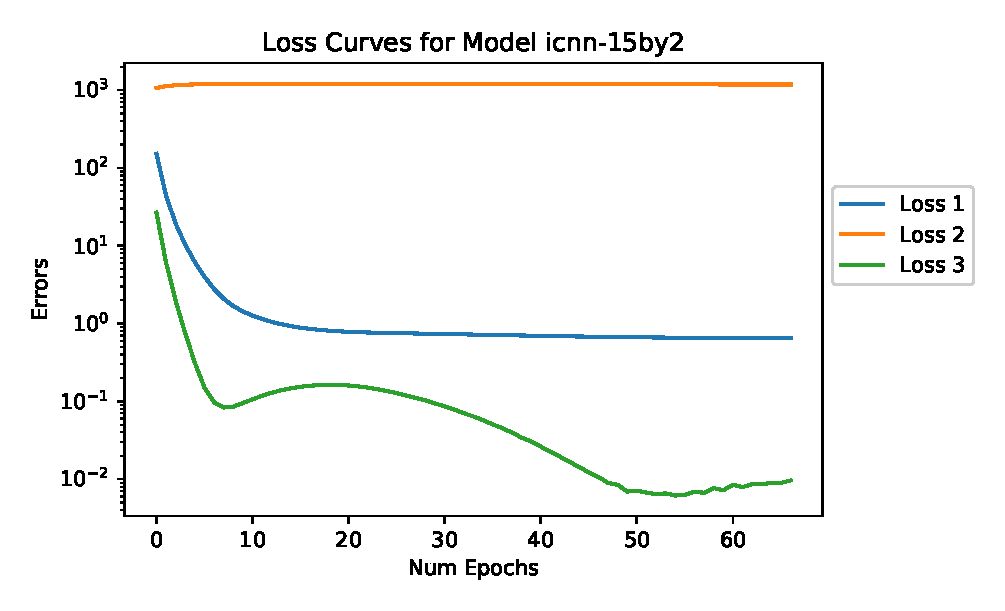
\includegraphics[width = 0.48\textwidth]{icnn15by2}}
	\subfigure[ECNN-15by5]{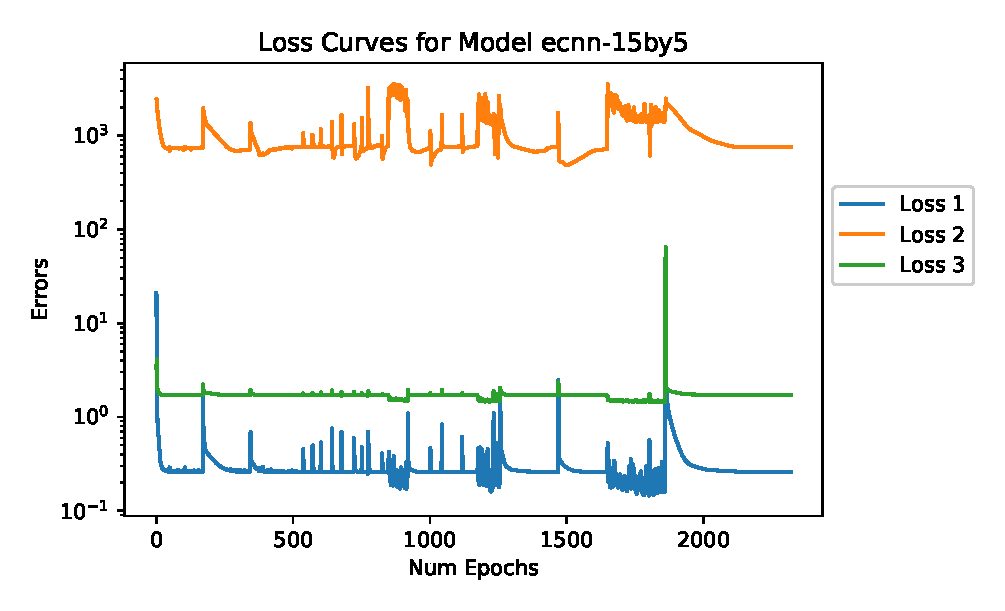
\includegraphics[width = 0.48\textwidth]{ecnn15by5}}
	\subfigure[ICNN-15by5]{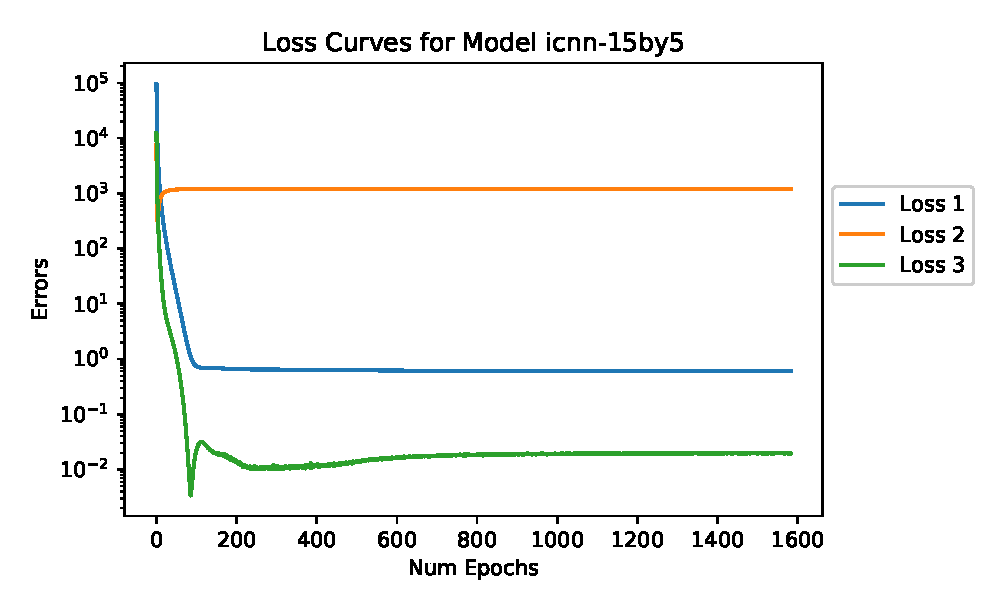
\includegraphics[width = 0.48\textwidth]{icnn15by5}}
	\subfigure[ECNN-15by10]{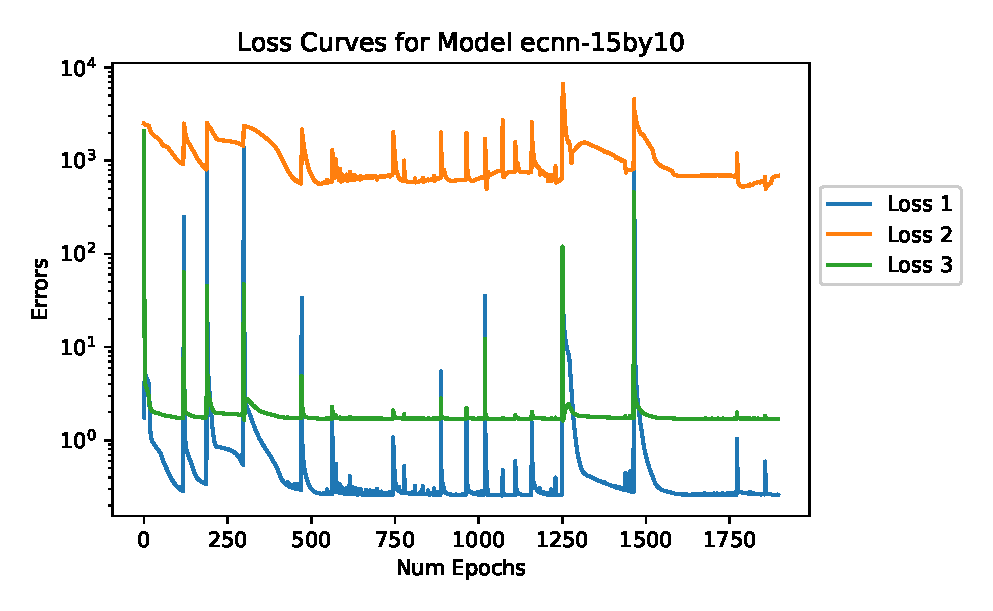
\includegraphics[width = 0.48\textwidth]{ecnn15by10}}
	\subfigure[ICNN-15by5]{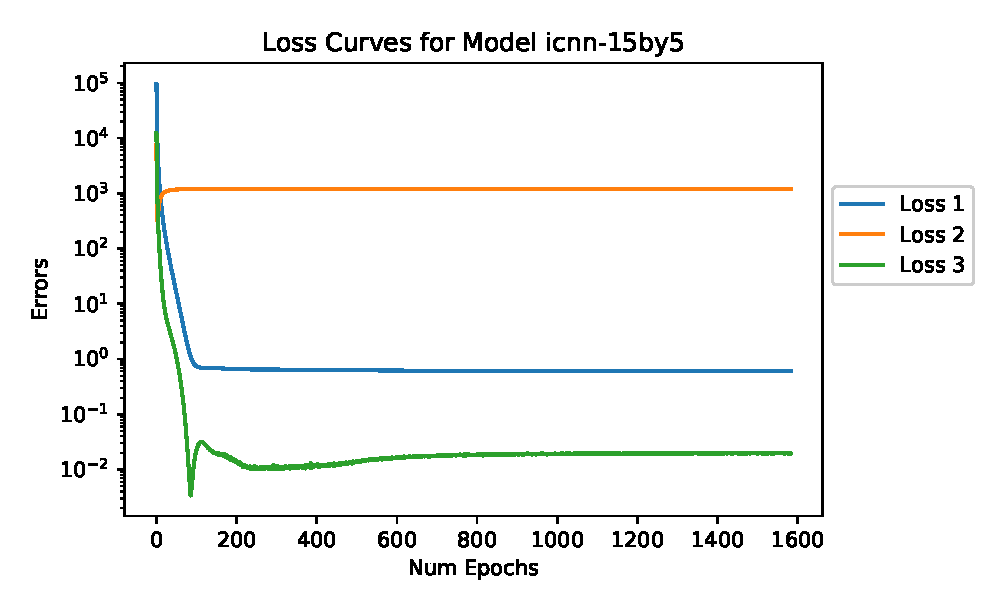
\includegraphics[width = 0.48\textwidth]{icnn15by5}}
	%\subfigure[u]{\includegraphics[width= 0.48\textwidth]{M2_data_driven_errbysize_u_new.eps}}
	%\subfigure[h]{\includegraphics[width = 0.48\textwidth]{M2_data_driven_errbysize_h_new.eps}}
\end{figure}


\subsection{Train and Test Error Performance}

\begin{table}[H]

\begin{tabular}{lrrrrrrr}
	\toprule
	{} &     Size &   RMSE h &   RMSE u &  RMSE u0 &  RMSE u1 &  RMSE alpha &  Num NegDef \\
	NetID     &          &          &          &          &          &             &             \\
	\midrule
	L1\_S15x2  & 5.26e+02 & 2.90e-01 & 3.34e-01 & 3.35e-01 & 3.33e-01 &    1.75e-01 &    0.00e+00 \\
	L1\_S15x5  & 1.25e+03 & 2.94e-01 & 3.39e-01 & 3.39e-01 & 3.38e-01 &    7.13e-02 &    0.00e+00 \\
	L1\_S15x10 & 2.45e+03 & 4.31e-01 & 3.18e-01 & 3.24e-01 & 3.10e-01 &    3.83e-01 &    5.20e+03 \\
	\bottomrule
\end{tabular}
\end{table}

\begin{table}[H]
\begin{tabular}{lrrrrrrr}
	\toprule
	{} &     Size &   RMSE h &   RMSE u &  RMSE u0 &  RMSE u1 &  RMSE alpha &  Num NegDef \\
	NetID     &          &          &          &          &          &             &             \\
	\midrule
	L1\_S15x2  & 5.26e+02 & 2.90e-01 & 3.34e-01 & 3.35e-01 & 3.33e-01 &    1.73e-01 &    0.00e+00 \\
	L1\_S15x5  & 1.25e+03 & 2.94e-01 & 3.39e-01 & 3.39e-01 & 3.38e-01 &    7.05e-02 &    0.00e+00 \\
	L1\_S15x10 & 2.45e+03 & 4.31e-01 & 3.18e-01 & 3.24e-01 & 3.10e-01 &    3.80e-01 &    5.21e+02 \\
	\bottomrule
\end{tabular}

\caption{ECNN Train Data Error Summary}
\end{table}

\begin{table}[H]
\begin{tabular}{lrrrrrrr}
	\toprule
	{} &     Size &   RMSE h &   RMSE u &  RMSE u0 &  RMSE u1 &  RMSE alpha &  Num NegDef \\
	NetID     &          &          &          &          &          &             &             \\
	\midrule
	L1\_S15x2  & 5.30e+02 & 7.14e-01 & 5.36e-01 & 4.38e-08 & 7.83e-01 &    9.93e-01 &    0.00e+00 \\
	L1\_S15x5  & 1.25e+03 & 6.49e-01 & 4.74e-01 & 4.64e-08 & 6.93e-01 &    9.89e-01 &    0.00e+00 \\
	L1\_S15x10 & 2.46e+03 & 4.54e-01 & 1.45e-01 & 7.79e-08 & 2.11e-01 &    9.30e-01 &    0.00e+00 \\
	\bottomrule
\end{tabular}

\caption{ICNN 2D-Test Data Error Summary}
\end{table}

\begin{table}[H]
	
\begin{tabular}{lrrrrrrr}
	\toprule
	{} &     Size &   RMSE h &   RMSE u &  RMSE u0 &  RMSE u1 &  RMSE alpha &  Num NegDef \\
	NetID     &          &          &          &          &          &             &             \\
	\midrule
	L1\_S15x2  & 5.30e+02 & 7.14e-01 & 5.36e-01 & 4.47e-08 & 7.83e-01 &    9.85e-01 &    0.00e+00 \\
	L1\_S15x5  & 1.25e+03 & 6.49e-01 & 4.74e-01 & 4.58e-08 & 6.93e-01 &    9.80e-01 &    0.00e+00 \\
	L1\_S15x10 & 2.46e+03 & 4.54e-01 & 1.45e-01 & 7.59e-08 & 2.11e-01 &    9.21e-01 &    0.00e+00 \\
	\bottomrule
\end{tabular}

\caption{ICNN Train Data Error Summary}
\end{table}




\end{document}